\chapter{Volume Average Method}
\label{ch:vans}

\chapquote{Do not worry about your difficulties in mathematics; I can assure you that mine are still greater.}{Letter to junior high school student Barbara Wilson, \\ January 7, 1943}{Albert Einstein}

\section{Introduction}

We have already said in the previous chapter that we use the volume averaging method to scale up the fluid equations, valid in the microscopic spaces of the porous medium, in order to find a macroscopic description that is valid everywhere in the porous medium domain (not only in the fluid phase).
Theoretical aspect of the volume averaging method applied to fluid in porous media can be found in \citet{whitaker2013method}, \citet{whitaker1986flow}, \citet{whitaker1996forchheimer}, \citet{quintard1994transport1}, \citet{quintard1994transport2}, \citet{quintard1994transport3}, \citet{quintard1994transport4}, \citet{quintard1994transport5} and many others contributions that are introduced in the next chapter.
In the following paragraph we describe the various stages necessary in calculating the local average version of equations \eqref{eq:NS}.

\section{Homogenization procedure}
The mathematical method of volume averaging is based on some fundamental stages that one should follow in order to retrieve the homogenized version of the equations.
The main steps are:
\begin{itemize}
\item Definition of the averaging operator
\item Use of theorems that permits to interchange the derivation and averaging operations
\item Decompose the fields in an "average plus perturbation" manner
\item Assume (based on the problem characteristics) some length-scales constraint that help to simplify and define a local closure  problem
\end{itemize}

Such schema is graphically resumed in \citet{paez2017macroscopic} and \citet{davit2013homogenization}; a similar flowchart of the complete overall procedure is showed in figure \ref{fig:schema_vans_homo}.

\begin{figure}[h!]
	\centering
	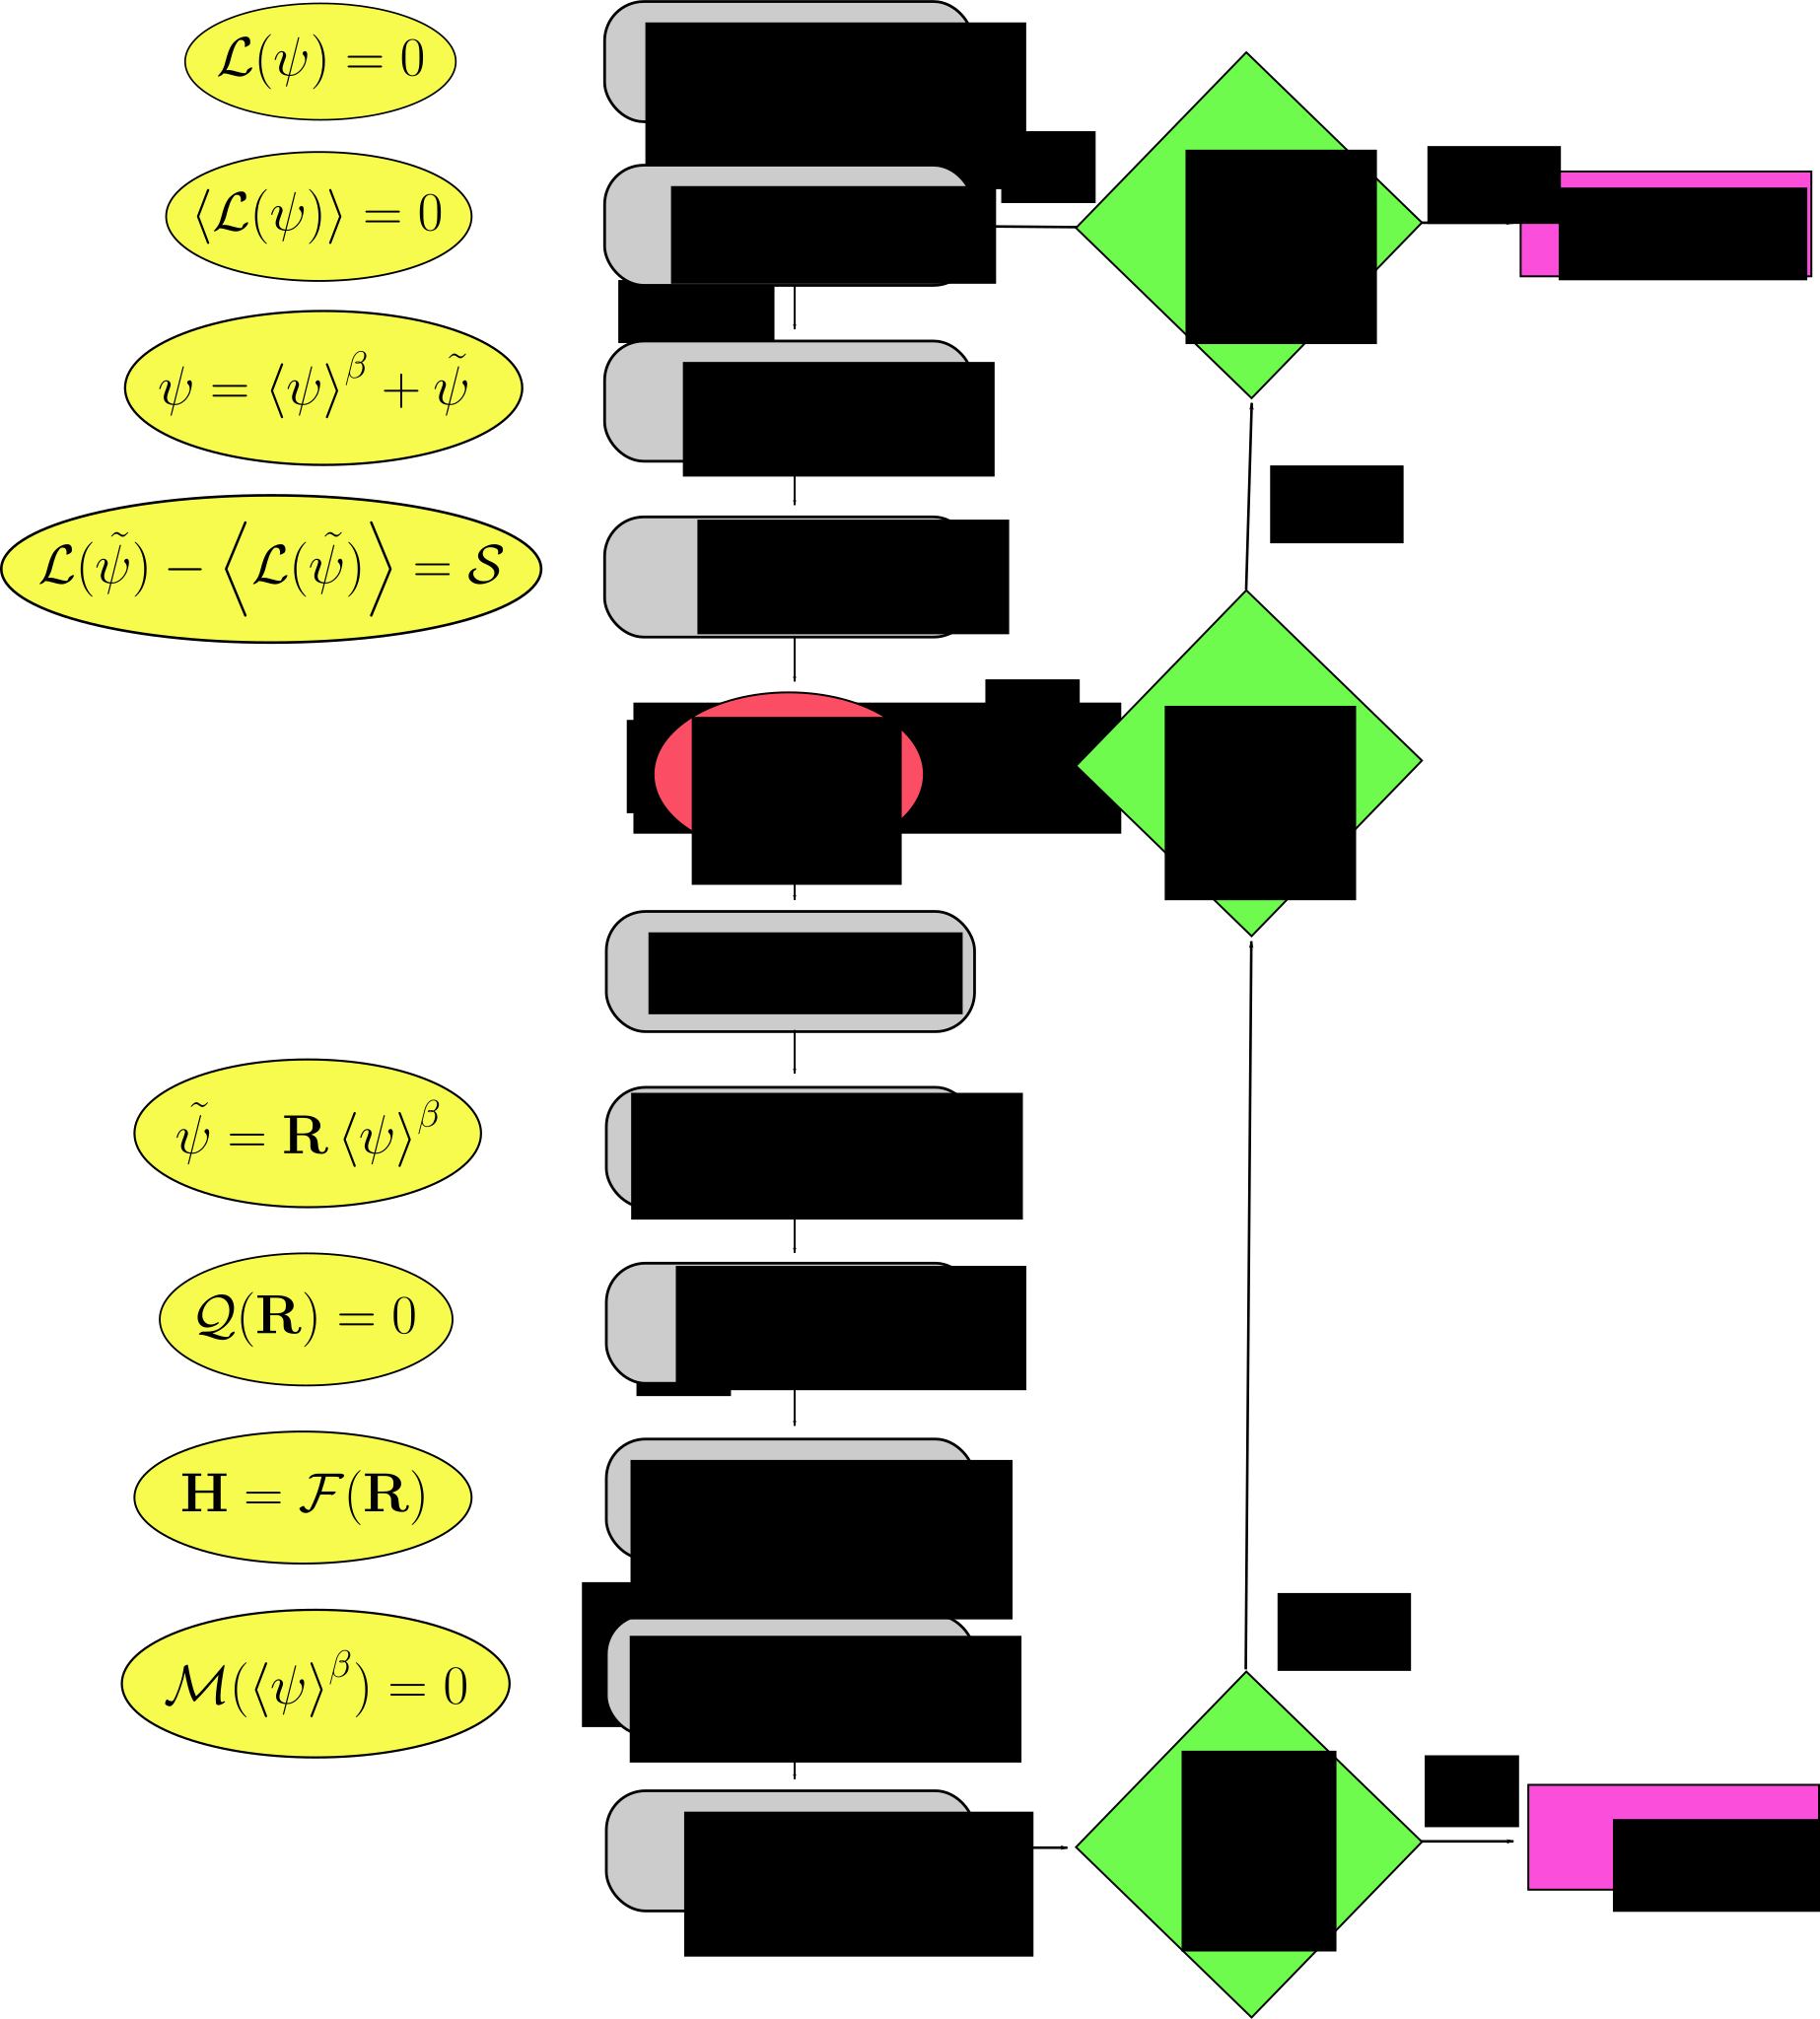
\includegraphics[width=0.95\textwidth,height=0.95\textheight,keepaspectratio]{chapter_2/figure/schema}
	\caption{Illustration of the volume average homogenization procedure. Image adapted from \citet{davit2013homogenization}}
	\label{fig:schema_vans_homo}
\end{figure}

\section{Derivation of VANS equations for 3D incompressible fluids}
The dynamic of the fluid phase (indicated with the subscript $\beta$), inside and above the porous medium, is governed by the Navier-Stokes equation for incompressible Newtonian fluid:

\begin{eqnarray}
	\begin{cases}
		\dfrac{\partial \vb}{\partial t} + \vb \cdot \nabla \vb = -\frac{1}{\rho_{\beta}} \nabla \pb + \nub \nabla^2  \vb  \\
		\nabla \cdot \ws = 0 \\
		\vb = \ws \qquad \text{at} \; A_{\beta\sigma}
	\end{cases}
\label{eq:NS}
\end{eqnarray}\\

where $\vb$, $\pb$, $\rho_{\beta}$ and $\nub$ stand, respectively, for  the velocity, the pressure, the density and the kinematic viscosity of the fluid.
The interface between the fluid and the solid is indicated as $A_{\beta\sigma}$, in which the no-slip condition for the velocity apply.
In the above boundary condition $\ws$ is velocity of the solid phase.
Initial condition should also be specified in order to solve the system, but they do not take active part in the homogenization procedure.
The next sections shows how to average this equations using the volume average method.

\subsection{Definition of the averaging operators}
Figure \ref{fig:rev} show the schematics of the internal structure of a fibrous porous medium; all the quantities needed in order to develop our mathematical approach are also indicated.
The continuous lines in the figure are used to indicate the shape of the volume used in the average operators, $V|_{\mathbf{x}}$ indicate the overall volume with centroid $\mathbf{x}$ and $V_{\beta}|_{\mathbf{x}}$ indicate the volume occupied of the only fluid phase inside the same volume.
The coordinate $\mathbf{r} = \mathbf{x} +\mathbf{y}$ represent the centroid of a possible volume in which one can compute the average quantities, the boundaries of the same volume are indicated with dotted lines.

\begin{figure}[h!]
	\centering
	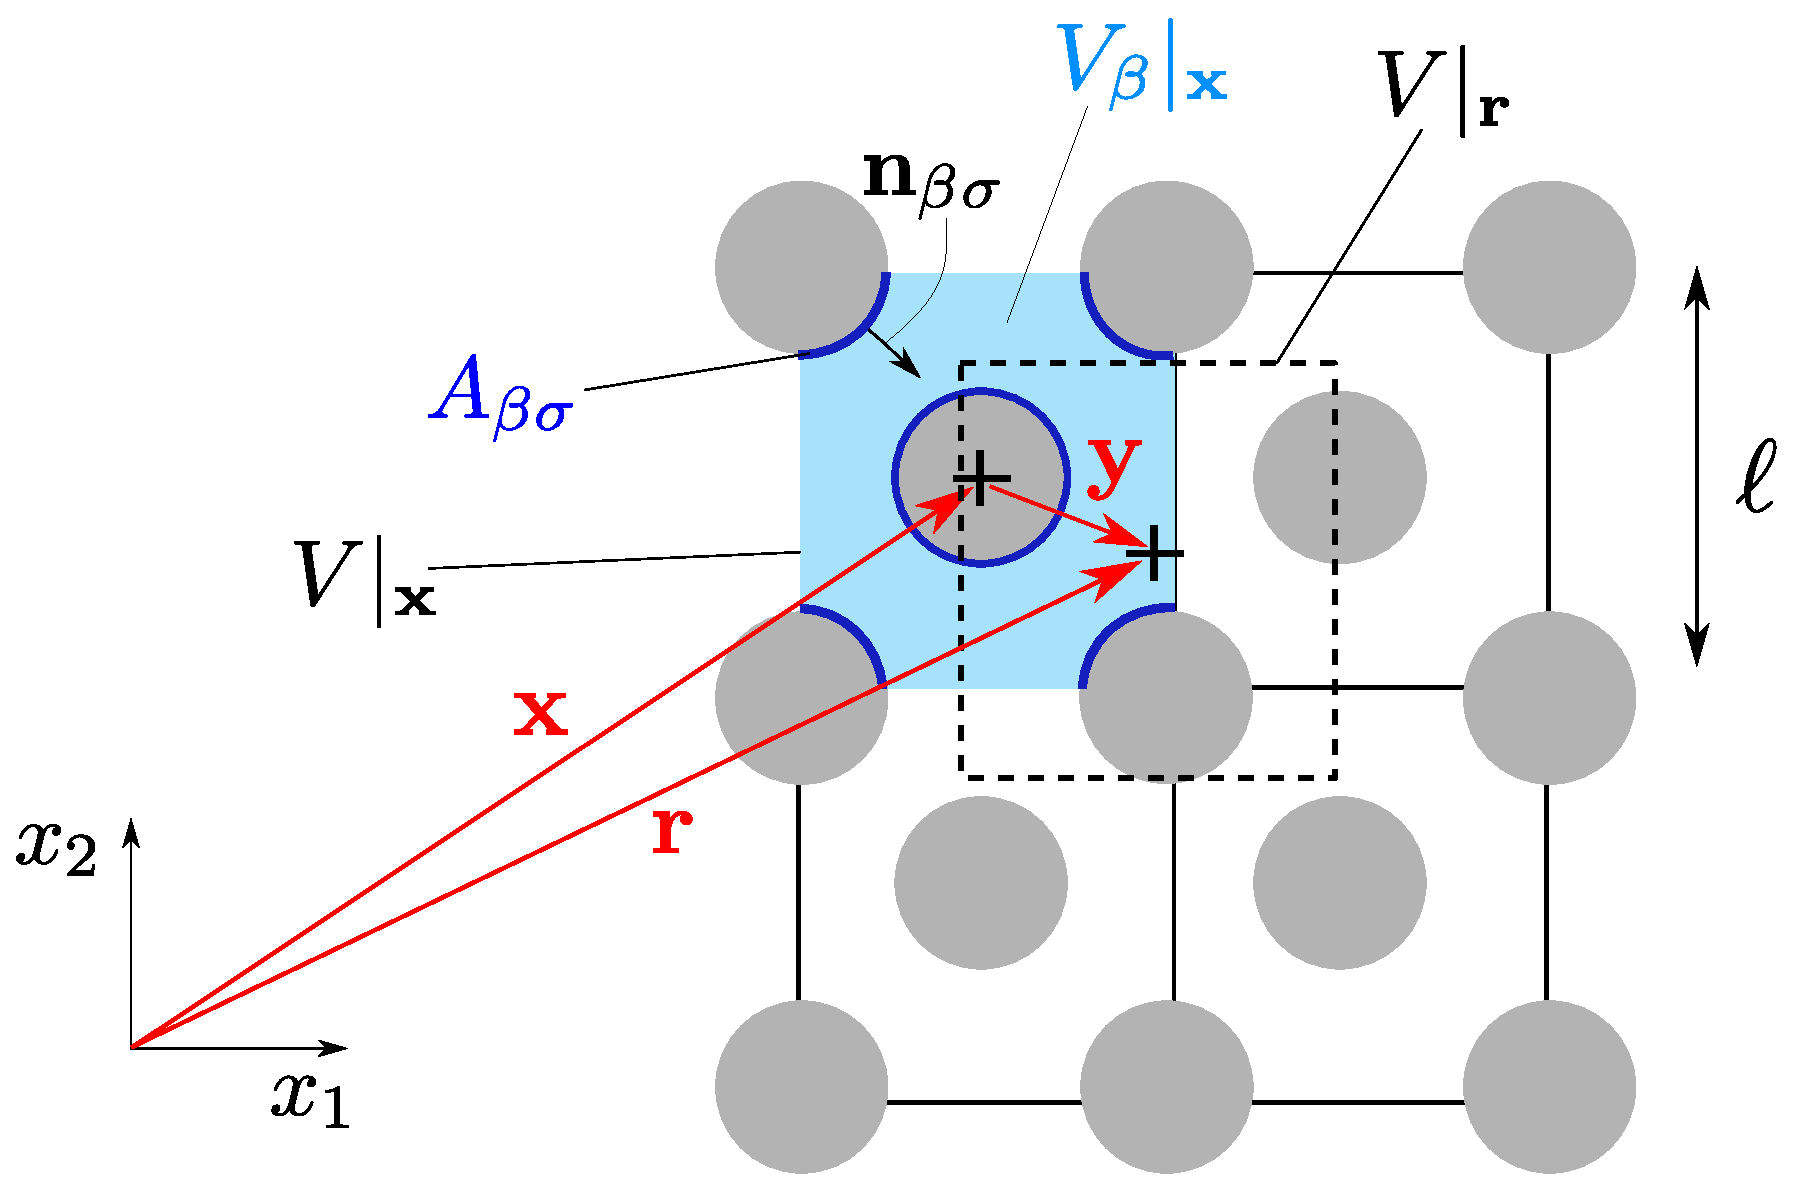
\includegraphics[width=0.7\linewidth]{chapter_2/figure/REV}
	\caption{A graphic representation of the averaging volumes and interfaces in case of fibrous (ordered) porous media. In this example the fibers are in staggered arrangement. The edges of the volumes that have centroid position $\mathbf{x}$ are shown in continuous lines and the ones with centroid $\mathbf{r}$ are shown in dotted lines.}
	\label{fig:rev}
\end{figure}

Let $\psi_{\beta}$ be a an arbitrary order tensors (scalar, vector or second order tensor) defined in the fluid phase of the volume $V$ with $x$ as centroid coordinates.
We define two different volume averaging operators; the \textit{intrinsic average} indicated as $\meani{.}$ reads:

\begin{equation}
	\meani{\psi_{\beta}}|_{\mathbf{x}} = \dfrac{1}{\volb(\mathbf{x})} \int_{\volb(\mathbf{x})}  m(\mathbf{y}) \psi_{\beta}(\mathbf{x}+\mathbf{y}, t) d \, \volb,
	\label{eq:avg_intrinsic}
\end{equation}

where $m$ is a weight function defined on $V$ and $\mathbf{y}$ is the relative position vector with respect to the centroid $\mathbf{x}$ of the averaging volume $\volb$.

The second one is the \textit{superficial average} indicated with $\means{}$:
\begin{equation}
	\means{\psi_{\beta}}|_{\mathbf{x}} = \dfrac{1}{V} \int_{\volb(\mathbf{x})} m(\mathbf{y}) \psi_{\beta}(\mathbf{x}+\mathbf{y}, t) d \, \volb,
	\label{eq:avg_superficial}
\end{equation}

The difference between the two formulation is that the former takes into account the actual fluid phase in averaging the filed instead of the pure size of the total volume.

In order to use a less heavy notation, the subscript $|_{\mathbf{x}}$ is dropped in the following procedure, but we keep in mind that the volume averaged quantities are explicitly dependent on the center position of the volume.
Either averaging operators are defined as a volume integral in which the integration domain size and shape should be chosen carefully in each different application; some more details on this choice are presented in the next paragraphs.

Inside the average operators we can further use a weight function ($m$), that has the aim to guarantee smooth volume averaged fields.
However the choice of its shape depends on the porous media geometry, and its size is connected to the chosen average volume.

In the sake of simplify the notation we consider the filter $m$ to be constant ($1/V$) inside the volume so we could drop it from the formulation of the average operators.
However any shape of the function $m$ can be used without formally change the final form of the averaged equation.

The porosity of a porous medium cell is defined as:
\begin{equation}
	\varepsilon = \dfrac{\volb}{V}
	\label{eq:porosity}
\end{equation}
which represent of how much fluid is actually present inside the averaging volume, and it also gives an indication of how packed are the fibers of our porous media.

Using the above definition is possible to express a relationship between the two averaging operators:
\begin{equation}
	\means{\psi_{\beta}} =  \varepsilon \meani{\psi_{\beta}}
	\label{eq:means_vs_meani}
\end{equation}

\subsection{Choice of shape and size of averaging volume and filter function}
\label{ch:filter}

The problem of choosing the right filter, for a give geometry of the porous medium, has been extensively studied by the series of works \citet{quintard1994transport1}, \citet{quintard1994transport2}, \citet{quintard1994transport3}, \citet{quintard1994transport4}, \citet{quintard1994transport5} and more recently generalized by \citet{davit2017technical}.

The authors above differentiate their results for ordered and disordered porous medium; and they show that in each case a specific size and shape of the filter (and the volume) is needed.
Sometimes in the following text we refer to the volume in which the average procedure is applied as REV, \textit{reference elementary volume}.
For disordered porous media a spherical volume is the most appropriate, and the REV size ($\ell_V$) should satisfy the length scale constraint:
$$
\ell_{\beta} \ll \ell_v \ll L
$$

Instead for ordered porous media the most appropriate shape is a cube with side:
$$
O(\ell_{\beta}) = \ell_V \ll L
$$
that can be reinterpreted as the separation of scale parameter in multiple scale analysis $\epsilon = \dfrac{\ell_{\beta}}{L} \ll 1$.

\citet{ochoa1995momentum} confirm the same length-scales constraints even in case of an interface between a free fluid and a porous medium.

The size of it ($\ell_v$) should be chosen with the above specifications, these length scales constraints assure that the volume is large enough that periodic boundary condition can be applied in the exterior of the volume but still be able to capture all the phenomena that take place at the micro-scale (scale $\ell_{\beta}$).
If the REV size is the correct one, increasing or decreasing its size, of a certain amount, should not change the averages quantities.

We have already said that the function can help to attenuate variation of the averaged fields due to geometrical fluctuations of the porous medium.
It has in fact the property of a low-pass filter for the perturbations fields.

The filter function can plays an important role also in the interpretation of the averaged equation in fact (as showed later) in order to retrieve a local form of the VANS equations we have to be able to make the statements:
\begin{equation}
\means{\means{\psi_{\beta}}|_{\mathbf{r}}}|_{\mathbf{x}} = \means{\psi_{\beta}}|_{\mathbf{x}}
\label{eq:well_behaved}
\end{equation}
that is equivalent to say that the averaged fields contains small variations of at the micro-scale (inside the averaging volume $V$).
In order to satisfy this requirement certain filter choices can perform better than others, although the same conclusion can be derived from the length-scales constraints.
In appendix \ref{ch:appendix_a} at the end of this chapter we further explain the details of the approximation needed to derive equations \ref{eq:well_behaved}.

For disordered porous medium the \textit{hat function} filter $m^{\sqcap}$ which has the form:
\begin{eqnarray}
	m^{\sqcap}(\mathbf{y}) 
	\begin{cases}
		\dfrac{1}{V} \qquad |\mathbf{y}| \leqslant r_0\\
		0 \qquad |\mathbf{y}|> r_0
	\end{cases}
\end{eqnarray}
can be used to produce smooth averaged fields.

Instead for ordered porous medium the literature show that triangle shaped functions called \textit{cellular filter}  $m^{\bigtriangleup}$  performs better:
\begin{eqnarray}
m^{\bigtriangleup}(\mathbf{y}) 
\begin{cases}
(\ell_{beta}/2 - |\mathbf{y}|) \qquad |\mathbf{y}| \leqslant r_0\\
0 \qquad |\mathbf{y}|> r_0
\end{cases}
\end{eqnarray}

Whichever is the choice on the $m$ shape, \citet{davit2017technical} has re-formulated recently the required hypothesis that a $m$ function should satisfy; without entry in the details (that is beyond the aim of this paragraph) we present some of the most important generalizations from the above works that should apply to any choice of the function $m$:
\begin{itemize}
	\item be normalized in as: $\int_{\volb}  m(\mathbf{y}) \; d\volb = 1$
	\item have compact support 
	\item $m*\psi_{\beta} \in C^{k}$ where $k$ represent the order of the closure
	\item $(m \, y^j)*\psi_{\beta}
	\begin{cases}
	0 \qquad if \quad j \; odd\\
	const  \qquad if \quad j \; even
	\end{cases}$
\end{itemize}

In the last requirement we have used the fact that the average operation can also be defined as a convolution product between the filter function and the flow field quantities, \citet{marle1982macroscopic}:
$$
\means{\psi_{\beta}}|_{\mathbf{x}} = \dfrac{1}{V} \int_{\volb(\mathbf{x})} m(\mathbf{y}) \psi_{\beta}(\mathbf{x}+\mathbf{y}, t) d \, \volb = m*\psi_{\beta}
$$

Even though we have shown the importance of the filter function shape, it should be clear that older literature works that had implicitly used the $m^{\sqcap}$ are not wrong, even in case of periodic ordered porous media.
In fact if we assume that the field are well behaved (even without checking if the filter or the REV size are the good one) we assume that the equation \eqref{eq:well_behaved} olds and that some simplifications of the averaging operators are permitted.
This permits us to finally find a closed local form of the equation and possibly use the good filter a posteriori to smooth the fields.
However neglecting the use of the proper filter can induce some problem on the interpretations of the averaged fields (as \citet{quintard1994transport1} show for the example case of hydrostatic pressure); so particular care should be used especially when making comparison to experiments.

In the following derivation of the equation we do not formally include any filter function inside the averaged operators in order to not make the notation heavier.
However we indicate in the following text where this hypothesis on the filter is formally needed to derive the equation.

\subsection{Theorems involving derivatives of spatial averaged quantities}

In this paragraph we report some the theorems related to the volume averaging technique. The purpose to these theorems is to invert the sequence of the  derivative and volume average operation.

\begin{theorem}[Spatial averaging theorem]
Let $\psi_{\beta}$ be a scalar quantity defined in the fluid phase $\beta$, then:

	\begin{equation}
		\means{\nabla \psi_{\beta}} = \nabla \means{\psi_{\beta}} + \dfrac{1}{V} \int_{A_{\beta \sigma}} \psi_{\beta} \nbs   \;dA
			\label{th:spat_avg}
	\end{equation}
\end{theorem}

In the above $\means{\psi_{\beta}}$ is evaluated at $\mathbf{x}$ and the operator $\nabla$ express the differentiation operation in respect to $\mathbf{x}$ also.

\begin{corollary}[Vector form of \eqref{th:spat_avg}]
	The vector form of the spatial averaging theorem is given by:
	
	\begin{equation}
	\means{\nabla \cdot \boldsymbol{\psi}_{\beta}} = \nabla \cdot \means{ \boldsymbol{\psi}_{\beta}} + \dfrac{1}{V} \int_{A_{\beta \sigma}}  \boldsymbol{\psi}_{\beta} \cdot \nbs \;dA
			\label{th:vec_spat_avg}
	\end{equation}
\end{corollary}

\begin{corollary}
	Applying the theorem \eqref{th:spat_avg} to a constant field $\psi_{\beta} = 1$ we obtain:
	
	\begin{equation}
		\nabla \varepsilon = - \int_{A_{\sigma \beta}} \nbs d \, A,
	\end{equation}
\end{corollary}


\begin{theorem}[Reynolds transport theorem]
	Let $\psi_{\beta}$ be a scalar quantity defined in the fluid phase $\beta$, then:
	
	\begin{equation}
	\dfrac{\partial}{\partial t} \int_{\volb(t)} \psi_{\beta} \; dV =  \int_{\volb(t)} \dfrac{\partial \psi_{\beta}}{\partial t} \; dV + \int_{A_{\beta \sigma}(t)} \psi_{\beta} (\ws \cdot \mathbf{n}_{\beta \sigma} ) \;dA,
	\label{th:transport}
	\end{equation}
	
	where $\ws$ is the point velocity of the solid-fluid interface $A_{\beta \sigma}$.
\end{theorem}

The three theorems and the corollary are indispensable to develop the closed form of the equations.
One interesting thing to pay attention is that the theorems switch the average and derivative operation but always introduces a non local integral term.

\subsection{Averaged continuity equations}
We start by finding the averaged version of the continuity equation in \eqref{eq:NS}:

\begin{equation}
\means{\nabla \cdot \vb}   = 0
\label{eq:superf_avg_cont}
\end{equation}

Applying theorem \eqref{th:spat_avg} to the previous equation we get:
$$
\means{\nabla \cdot \vb} = \nabla \cdot \means{\vb} + \dfrac{1}{V} \int_{A_{\beta \sigma}}  \vb \cdot \nbs \;dA
$$
The boundary condition at the interface ($\ws = \vb$) imply that the integral above can be modified: 
$$=\nabla \cdot \means{\vb} + \dfrac{1}{V} \int_{A_{\beta \sigma}}  \ws \cdot \nbs \;dA$$
Now we rewrite the last term as if it was a result of the Reynolds transport theorem applied to a constant unitary scalar field:
$$=\nabla \cdot \means{\vb} + \derp{}{t} \dfrac{1}{V} \int_{\volb} \;dV  - \dfrac{1}{V} \int_{\volb} \derp{1}{t} \;dV $$
This results can be simplified; in fact the last integral is zero due to the time derivation of a constant field. The first term can be further developed, obtaining finally the averaged continuity equation \eqref{eq:avg_1}.

\begin{equation}
\nabla \cdot \means{\vb} + \derp{\varepsilon}{t} =0
\label{eq:avg_1}
\end{equation}


\subsection{Averaged momentum equations}
In this paragraph we compute the average version of the momentum equation in \eqref{eq:NS}:

\begin{equation}
\dfrac{\partial \vb}{\partial t} + \nabla \cdot (\vb\vb) = -\frac{1}{\rho_{\beta}} \nabla \pb + \nub \nabla^2  \vb
\label{eq:mom_1}
\end{equation}

In order to keep the procedure readable we show the development of each term separately, in the same order as they appear in equation \eqref{eq:mom_1}.

\subsubsection{Temporal derivative term}
Using theorem \eqref{th:transport} we can rewrite the first term of the equation as:

\begin{equation}
\means{\derp{\vb}{t}} = \derp{\means{\vb}}{t} -\dfrac{1}{V} \int_{A_{\beta \sigma}(t)} (\ws \cdot \nbs ) \vb \;dA,
\end{equation}

\subsubsection{Convective term}
Theorem \eqref{th:vec_spat_avg} applied to the convective term gives us:

\begin{equation}
\means{\nabla \cdot (\vb\vb)} = \nabla \cdot \means{\vb \vb} + \dfrac{1}{V} \int_{A_{\beta \sigma}}  (\vb \vb) \cdot \nbs \;dA,
\end{equation}

The boundary condition at the interface ($\ws = \vb$) imply that the integrals inside the convective and temporal part are equals, so the total left end side of the momentum equation became:

\begin{equation}
\derp{\means{\vb}}{t} + \nabla \cdot \means{\vb \vb}
\label{eq:lhs}
\end{equation}

\subsubsection{Pressure term}
The pressure term is also expanded using theorem \ref{th:spat_avg}:

\begin{equation}
\means{-\dfrac{1}{\rho_{\beta}} \nabla \pb } = -\dfrac{1}{\rho_{\beta}} \nabla \means{\pb} -\dfrac{1}{V} \int_{A_{\beta \sigma}} \dfrac{\pb}{\rho_{\beta}} \nbs \;dA,
\end{equation}

\subsubsection{Diffusion term}
Here we fist use the identity $\nabla^2 = \nabla \cdot (\nabla)$ (laplacian = div(grad)), then we apply the theorem \ref{th:vec_spat_avg} directly to this expansion to get:

\begin{equation}
\means{\nub\nabla^2 \vb} = \means{\nub\nabla \cdot \nabla \vb} = \nabla \cdot \means{\nub\nabla \vb} +\dfrac{1}{V} \int_{A_{\beta \sigma}}  \nub \nabla \vb \cdot \nbs \;dA,
\label{eq:4_1}
\end{equation}

Now re-using the theorem \ref{th:vec_spat_avg} on $\means{\nabla \vb}$:

\begin{eqnarray}
	\eqref{eq:4_1} &=& \nabla \cdot \nub \nabla \means{\vb} + \nabla \cdot \left( \dfrac{1}{V} \int_{A_{\beta \sigma}} \nbs \cdot \nub \vb \;dA \right) + \dfrac{1}{V} \int_{A_{\beta \sigma}} \nbs \cdot \nub \nabla \vb \;dA = \nonumber \\
	&=& \nub\nabla^2 \means{\vb} +  \nabla \cdot \left( \dfrac{1}{V} \int_{A_{\beta \sigma}} \nbs \cdot \nub \vb \;dA \right) + \dfrac{1}{V} \int_{A_{\beta \sigma}} \nbs \cdot \nub \nabla \vb \;dA  = \nonumber \\
	&& \text{using Gauss theorem on the second term} \nonumber \\
	&=& \nub\nabla^2 \means{\vb} +  \nabla \cdot \left( \dfrac{1}{V} \int_{\volb} \nabla \cdot \nub \vb d\volb \right) + \dfrac{1}{V} \int_{A_{\beta \sigma}} \nbs \cdot \nub \nabla \vb \;dA = \nonumber \\
	&& \text{which is zero due to the continuity equation} \nonumber \\
	&=& \nub\nabla^2 \means{\vb} + \dfrac{1}{V} \int_{A_{\beta \sigma}} \nbs \cdot \nub \nabla \vb \;dA
\end{eqnarray}

\Red{The above use of the Gauss theorem, to prove that the first integral term is zero, can be bypassed in case of rigid porous media. Which due to the b.c. at the fluid-solid is zero.}

Before continue the development we group all the various terms together:

\begin{eqnarray}
&& \derp{\means{\vb}}{t} + \nabla \cdot \means{\vb \vb} = -\dfrac{1}{\rho_{\beta}} \nabla \means{\pb} + \nub\nabla^2 \means{\vb} + \nonumber \\
&& +\dfrac{1}{V} \int_{A_{\beta \sigma}} \left( -\dfrac{\pb}{\rho_{\beta}} \mathbf{I} + \nub \nabla \vb  \right)\cdot \nbs \;dA \nonumber \\
\label{eq:mom_2}
\end{eqnarray}

This is still not the averaged version of the momentum equation, since it has the presence of the non-homogeneous term $\means{\vb\vb}$ and the integral term still has the point variables inside.
In the next section these we show how to thereat these two terms in order make them function of the only averaged quantities.

\subsection{Length scale decomposition}
In order to finally get the average version of the problem \eqref{eq:NS} we make use of the decomposition proposed by \citet{gray1975derivation}:

\begin{equation}
\psi_{\beta}(\mathbf{r},t) = \meani{\psi_{\beta}}|_{(\mathbf{r},t)} + \tilde{\psi}_{\beta}(\mathbf{r},t)
\label{eq:gray}
\end{equation}

where $\tilde{\psi}_{\beta}$ is the microscopic scale contribution to add at the intrinsic volume average quantity $ \meani{\psi_{\beta}}$ (that is representative of the macro-scale $L$) to obtain the point value of the considered quantity $\psi_{\beta}$.
This decomposition has been introduced in order to separate the different scales of the spatial variation of the fields, and so separate the low frequencies from the high one.

If the hypothesis of that this division holds, it is possible to demonstrate that the average value of the perturbation field is null (the paragraph \ref{ch:appendix_a} specifically address the hypothesis behind this result):
$$
\means{\tilde{\psi}_{\beta}} = \means{\psi_{\beta}} - \means{\meani{\psi_{\beta}}} \approx \means{\psi_{\beta}} -\varepsilon \meani{\psi_{\beta}} = 0
$$


Using the above results we can modify the non-homogeneous term in equation \eqref{eq:mom_2}:

\begin{equation}
\means{\vb\vb} = \meani{\means{\vb}\meani{\vb}} +2\means{\meani{\vb}\vbt} +\means{\vbt \vbt} = \varepsilon \meani{\vb}\meani{\vb} +\means{\vbt\vbt}
\label{eq:dec_1}
\end{equation}

For each integral term of \ref{eq:mom_2} we also apply the same field decomposition:

\begin{eqnarray}
\dfrac{1}{V} \int_{A_{\beta \sigma}}  -\dfrac{\pb}{\rho_{\beta}} \nbs \;dA &=& \dfrac{1}{V} \int_{A_{\beta \sigma}}  -\dfrac{1}{\rho_{\beta}} \left(\meani{\pb}  + \pbt\right) \nbs \;dA = \nonumber \\
&=& +\dfrac{1}{\rho_{\beta}}\nabla\varepsilon \meani{\pb} - \dfrac{1}{V} \int_{A_{\beta \sigma}} \dfrac{\pbt}{\rho_{\beta}} \nbs \;dA
\end{eqnarray}


\begin{eqnarray}
\dfrac{1}{V} \int_{A_{\beta \sigma}} \nub \nabla \vb \cdot \nbs \;dA &=& \dfrac{1}{V} \int_{A_{\beta \sigma}} \nub \nabla (\meani{\vb} +\vbt) \cdot \nbs \;dA =  \nonumber \\
&=& - \nub \nabla \varepsilon \nabla \meani{\vb} + \dfrac{1}{V} \int_{A_{\beta \sigma}} \nub \nabla \vbt \cdot \nbs \;dA
\end{eqnarray}

%\begin{eqnarray}
%&&\nabla \cdot \left( \dfrac{1}{V} \int_{A_{\beta \sigma}} \nbs \cdot \nub \vb \;dA \right) = \nabla \cdot \left( \dfrac{1}{V} \int_{A_{\beta \sigma}} \nbs \cdot \nub (\meani{\vb} +\vbt) \;dA \right) =  \nonumber \\
%&=& -\nabla \cdot \left( \nub \meani{\vb} \nabla \varepsilon \right) + \dfrac{1}{V} \nabla \cdot \left(\int_{A_{\beta \sigma}}  \nub \nbs \vbt \;dA \right) =  \nonumber \\
%&=& -\nub  \nabla  \meani{\vb} \nabla \varepsilon -\nub \meani{\vb} \nabla^2 \varepsilon + \dfrac{1}{V} \nabla \cdot \left(\int_{A_{\beta \sigma}}  \nub \nbs \vbt \;dA \right)
%\end{eqnarray}

The momentum equation now reads:

\begin{eqnarray}
\derp{\means{\vb}}{t} + \nabla \cdot (\varepsilon \meani{\vb}\meani{\vb}) + \nabla \cdot (\means{\vbt\vbt}) = -\dfrac{1}{\rho_{\beta}} \nabla \means{\pb} + \nub\nabla^2 \means{\vb} + \nonumber \\
\qquad \qquad - \nub \nabla \varepsilon \nabla \meani{\vb} +\dfrac{1}{\rho_{\beta}}\nabla\varepsilon \meani{\pb} +\dfrac{1}{V} \displaystyle\int_{A_{\beta \sigma}} \left( -\dfrac{\pbt}{\rho_{\beta}} \mathbf{I} + \nub \nabla \vbt  \right)\cdot \nbs \;dA
\label{eq:NS_2}
\end{eqnarray}

At this stage the momentum equation is not closed since it has the mixed presence of surface and intrinsic averaged quantities, and also perturbation fields.
In order to overcome this problems in the next section the intrinsic version of these equation is finally computed. 

\subsection{Intrinsic average form}
In order to get the intrinsic average formulation we use the relation \eqref{eq:means_vs_meani} to express surface averaged quantities in terms of intrinsic ones.

We first start withe the continuity equation that became:
$$
\nabla \cdot (\varepsilon\meani{\vb} ) + \derp{\varepsilon}{t}= 0
$$

For the momentum equation we start from the temporal derivative term that became:
$$
\derp{\means{\vb}}{t} = \derp{(\varepsilon\meani{\vb})}{t} = \derp{\varepsilon}{t}\meani{\vb} + \varepsilon \derp{\meani{\vb}}{t}
$$

Applying the same relation to the viscous term we get:

\begin{equation}
	\nabla^2 \means{\vb} = \nabla^2 \left( \varepsilon \meani{\vb} \right) = \varepsilon \nabla^2 \meani{\vb} + \meani{\vb} \nabla^2 \varepsilon +2 \nabla \varepsilon \nabla \meani{\vb}
\end{equation}

and the pressure one also transform into:

\begin{equation}
\nabla \means{\pb} = \nabla \left( \varepsilon \meani{\pb} \right) = \varepsilon \nabla \meani{\pb} + \meani{\pb} \nabla \varepsilon
\end{equation}

Putting now altogether:

\begin{eqnarray}
&& \derp{\varepsilon}{t}\meani{\vb} + \varepsilon \derp{\meani{\vb}}{t} + \nabla \cdot \left(\varepsilon \meani{\vb}\meani{\vb}\right)   + \nabla \cdot \left(\means{\vbt \vbt}\right) = \nonumber \\
&&= -\varepsilon \nabla \left(\dfrac{\meani{\pb}}{\rho_{\beta}}\right) - \dfrac{\meani{\pb}}{\rho_{\beta}} \nabla \varepsilon + \nub \varepsilon \nabla^2 \meani{\vb} + \nub \meani{\vb} \nabla^2 \varepsilon + 2 \nabla \varepsilon \nabla \meani{\vb} \nonumber \\
&&+\dfrac{1}{\rho_{\beta}}\nabla\varepsilon \meani{\pb} - \dfrac{1}{V} \int_{A_{\beta \sigma}} \dfrac{\pbt}{\rho_{\beta}} \nbs \;dA \nonumber \\
&&- \nub \nabla \varepsilon \nabla \meani{\vb} + \dfrac{1}{V} \int_{A_{\beta \sigma}} \nub \nabla \vbt \cdot \nbs \;dA
\end{eqnarray}

After the proper simplification we have the final versions of the Navier-Stokes system of equations \eqref{eq:NS} using intrinsic quantities:

\begin{eqnarray}
\begin{cases}
 \derp{\varepsilon}{t}\meani{\vb} + \varepsilon \derp{\meani{\vb}}{t} + \nabla \cdot \left(\varepsilon \meani{\vb}\meani{\vb}\right)   + \nabla \cdot \left(\means{\vbt \vbt}\right) =  \\
\qquad \qquad = -\varepsilon \nabla \left(\dfrac{\meani{\pb}}{\rho_{\beta}}\right) + \nub \varepsilon \nabla^2 \meani{\vb} +  \nabla \varepsilon \nabla \meani{\vb} + \nub \meani{\vb} \nabla^2 \varepsilon  \\
\qquad \qquad + \dfrac{1}{V} \displaystyle\int_{A_{\beta \sigma}} \left(-\dfrac{\pbt}{\rho_{\beta}} \mathbf{I}  + \nub \nabla \vbt \right)\cdot \nbs \;dA \\
 \nabla \cdot (\varepsilon\meani{\vb} ) + \derp{\varepsilon}{t}= 0 
\end{cases}
\label{eq:vans_mom_1}
\end{eqnarray}


First of all is important to pinpoint that the intrinsic momentum equation represent the force per unit volume, so it explicitly depends on the porosity of the medium that can change the unit volume size (this is why it has terms involving gradients of the porosity).
In application where porosity can vary spatially (like the interface of a porous medium) this formulation has the advantage to treat explicitly the interface non-homogeneities (further discussion of the interface treatment is presented in paragraph \ref{ch:interface}).

%Another difference between the superficial and the intrinsic formulation is in the continuity equation; we can observe that even in case of steady problem only the superficial velocity field is solenoidal.

The equation \eqref{eq:vans_mom_1} is also \textit{non-local} since it has volume average quantities and surface integrals.
This very terms need some explicit manipulation in order to get a close formulation of the above system.
In the next paragraphs we develop closure formulations of these terms. In order to do be clear we name these terms as \textit{sub-filter stresses} $\boldsymbol{\zeta}$ and \textit{microscopic force} at the fluid-solid interface $\mathbf{F}^m$:

$$
\boldsymbol{\zeta} = \nabla \cdot \left(\means{\vbt \vbt}\right)
$$

$$
\mathbf{F}^m =  \dfrac{1}{V} \int_{A_{\beta \sigma}} \left(-\dfrac{\pbt}{\rho_{\beta}} \mathbf{I}  + \nub \nabla \vbt \right)\cdot \nbs \;dA
$$

\section{Closure problems}

\subsection{Microscopic force $\mathbf{F}^m$}
The term $\mathbf{F}^m$ is referred as \textit{surface filter} since it is defined as an integral over the fluid-solid interface for the micro-scale fields; in this manner the perturbation fields are filtered out.

There is no simple representation for $\mathbf{F}^m$ if we include the terms that presents gradients of the porosity ($\nabla \varepsilon$).
Although since we are interested in developing a \textbf{local} closure problem, that will depend on the geometry of each REV, is possible to simplify these terms.
This means that the closure problems are not correct at the interface between a porous medium and a free fluid; but in the last chapter we show that even though we are indeed committing an error, we can still use the same closure problems and, still obtain good results.

In order to develop a closure problem we recall the decomposition by \citet{gray1975derivation}:
\begin{equation}
\psi_{\beta} = \meani{\psi_{\beta}} + \tilde{\psi}_{\beta}
\end{equation}

From the continuity equation valid at the microscopic scale, we subtract the continuity equation valid for the intrinsic average velocity:

$$
\nabla \cdot  \vb - \nabla \cdot  \meani{\vb} = 0
$$


expanding the first velocity with the decomposition above, and making the evident simplification, we obtain the continuity equation for the perturbations:

\begin{equation}
\nabla \cdot \vbt = 0 
\end{equation}


With the same procedure, we first dived the momentum equation in system \ref{eq:vans_mom_1} by the permeability $\varepsilon$, and then subtract them from the point equations obtaining:

\begin{eqnarray}
&&  \derp{\vbt}{t} + \vb \cdot \nabla \vbt + \vbt \cdot \nabla \meani{\vb}  = \nonumber \\
&&= -\nabla \left(\dfrac{\pbt}{\rho_{\beta}}\right) + \nub \nabla^2 \vbt - \varepsilon^{-1}\nabla \cdot  \means{\vbt \vbt} +  \varepsilon^{-1} \nabla \varepsilon \nabla \meani{\vb} + \varepsilon^{-1} \nub \meani{\vb} \nabla^2 \varepsilon \nonumber \\
&&- \dfrac{1}{\volb} \displaystyle\int_{A_{\beta \sigma}} \left(-\dfrac{\pbt}{\rho_{\beta}} \mathbf{I}  + \nub \nabla \vbt \right) \cdot \nbs \;dA
\label{eq:vans_mom_3}
\end{eqnarray}

Now in order to simplify the above equations we introduce these length-scale estimates:
$$ \vbt = O(\meani{\vb}), \qquad \nabla\vbt = O(\dfrac{\meani{\vb}}{\ell}), \qquad  \nabla \meani{\vb} = O(\dfrac{\meani{\vb}}{L}), \qquad \varepsilon = O(\delta) $$

where the last length scale estimates is based on the fact that the porosity varies on scale $\delta$ that is much greater than $\ell$, this means $\ell \ll \delta$. \citet{valdes2013velocity} and \citet{ochoa1995momentum} make this argument considering that $\delta$, in the case of an interface between a porous medium and a free fluid, is the size of the zone in which the porosity varies.
However is important to state that this assumption does not holds at the interface of all the porous media geometry (for ordered porous media $\varepsilon = O(\ell)$).
\citet{whitaker1996forchheimer} state clearly that there is no easy way to define a \textit{local} closure problem when the relation $\ell \ll \delta$ does not holds; in any case here we suppose it correct to fulfill the derivation of the local closure problem although we keep in mind this problem holds only far from region where the porosity field change (even if in the last chapter we show that relaxing this hypothesis still produce good results).

Continuing with the order estimates we can neglect some of the terms based on the estimation of different order of magnitude:
\begin{eqnarray}
\vb \cdot \nabla \vbt \gg \vbt \cdot \nabla \meani{\vb} \quad &\Rightarrow&  \quad O\left(\dfrac{\meani{\vb}}{\ell}\right) \gg O\left(\dfrac{\meani{\vb}}{L} \right) \\
\vb \cdot \nabla \meani{\vbt} \gg  \varepsilon^{-1} \nabla \cdot \left(\means{\vbt \vbt}\right)  \quad &\Rightarrow& \quad O\left(\dfrac{(\meani{\vb})^2}{\ell}\right) \gg O\left(\dfrac{(\meani{\vb})^2}{\delta} \right) \\
\derp{\vbt}{t} \ll \nub \nabla^2 \vbt  \quad &\Rightarrow&  \quad O\left(\dfrac{(\meani{\vb})^2}{\ell}\right) \gg O\left(\dfrac{(\meani{\vb})^2}{L} \right) 
\end{eqnarray}

In the last estimation we have assumed that the time scale associated respectively with the micro and macro-scale are $t = \dfrac{\ell}{\meani{\vb}}$ and $T =\dfrac{L}{\meani{\vb}}$.
This assumption imply the \textit{quasi-stationary} of the perturbation problem, and it is physically held by the fact that the perturbation problem can be considered steady from the macroscopic evolution perspective \citet{davit2013homogenization} and \citet{zhu2014study}.
The readers familiars with the multiples scales methods can notice that in the above simplifications we have neglected terms that contains the small parameter $\epsilon$ (or powers of this term), that is coherent with the theory in which only zero order terms are used in the local closure problem formulation.

The order of magnitude estimation leave use with:
\begin{eqnarray}
	\begin{cases}
		\vb \cdot \nabla \vbt = -\nabla \left(\dfrac{\pbt}{\rho_{\beta}}\right) + \nub \nabla^2 \vbt - \dfrac{1}{\volb} \int_{A_{\beta \sigma}} \left(-\dfrac{\pbt}{\rho_{\beta}} \mathbf{I}  + \nub \nabla \vbt \right) \cdot \nbs \;dA  \\
		\nabla \cdot \vbt = 0  \\
		\vbt = -\meani{\vb} \quad at \; A_{\beta \sigma}
	\end{cases}
\label{eq:vans_mom_}
\end{eqnarray}
that is indeed the transport equations system for the perturbation fields.

The above system is still defined on all the porous domain and so we would like to find a way to reduce its size and still obtain the same results.
Another issue with the above system is that it still contain some macroscopic terms that act as source; this micro-macro scale couplings would constrain us to solve the system on the overall domain for either the averaged and the fluctuations field, with no practical advantage over the point equations.
Although is possible to use Green function to solve the problem in this form \citet{wood2013volume}, we are interested in a \textit{local} closure problem.

This can be done restricting the solution region to a single REV, enforcing periodic boundary condition at the exterior of such volume.
Such hypothesis is consistent with periodic order porous media because we have already stated that the variations connected to mean averaged quantities can be neglected inside the REV (see paragraph \ref{ch:appendix_a}).
The problem stated in these manner became:

\begin{eqnarray}
\begin{cases}
\vb \cdot \nabla \vbt = -\nabla \left(\dfrac{\pbt}{\rho_{\beta}}\right) + \nub \nabla^2 \vbt - \dfrac{1}{\volb} \int_{A_{\beta \sigma}} \left(-\dfrac{\pbt}{\rho_{\beta}} \mathbf{I}  + \nub \nabla \vbt \right) \cdot \nbs \;dA  \\
\nabla \cdot \vbt = 0  \\
\vbt = -\meani{\vb} \quad at \; A_{\beta \sigma} \\
\pbt(\mathbf{x} +\ell_i) = \pbt(\mathbf{x}), \qquad \vbt(\mathbf{x} +\ell_i) = \vbt(\mathbf{x}), \qquad i=1,2,3 \\
\meani{\vbt} = 0
\end{cases}
\label{eq:vans_mom_2}
\end{eqnarray}

In the above problem the averaged condition $\meani{\vbt} = 0$ is used to make the solution unique, that otherwise will be defined up to a constant.

Now we introduce the closure variables $\mathbf{R}$, $\mathbf{r}$, for which we made the hypothesis that:
\begin{eqnarray}
&& \vbt(\mathbf{x}) = \mathbf{R}(\mathbf{x})  \cdot \meani{\vb}(\mathbf{x})  +\boldsymbol{\xi}(\mathbf{x})   \\
&& \pbt(\mathbf{x})  = \mub \mathbf{r}(\mathbf{x})  \cdot \meani{\vb}(\mathbf{x})  + \gamma(\mathbf{x})
	\label{eq:closure_viab_hp}
\end{eqnarray}
the above choice is just dictate from convenience.
Is very important to pinpoint that the last assumption is crucial since we imply a linear correlation between the micro and macro-scale fields.
Even if this dependence can be space dependent, it means that can vary in each point $x$ of the macroscopic space (this functional dependence will be further explored in chapter \ref{ch:4}).


Since we are free to define the tensor $\mathbf{R}$  and the vector $\mathbf{r}$ as we wish, we chose to define it by means of the following problem:

\begin{eqnarray}
	\begin{cases}
		\dfrac{\vb}{\nub} \cdot  \nabla \mathbf{R} = -\nabla \mathbf{r} + \nabla^2 \mathbf{R} - \dfrac{1}{\volb} \int_{A_{\beta \sigma}} \left(-\mathbf{r}\mathbf{I}  +  \nabla \mathbf{R} \right) \cdot \nbs \;dA  \\
		\nabla \cdot \mathbf{R} = 0  \\
		\mathbf{R} = \mathbf{I} \quad at \; A_{\beta \sigma} \\
		\mathbf{r}(\mathbf{x} +\ell_i) = \mathbf{r}(\mathbf{x}), \qquad \mathbf{R}(\mathbf{x} +\ell_i) = \mathbf{R}(\mathbf{x}), \qquad i=1,2,3 \\
		\meani{\mathbf{R}} = 0
	\end{cases}
\label{eq:R_problem}
\end{eqnarray}

With  $\mathbf{R}$ and $\mathbf{r}$ specified as above we can prove that $\boldsymbol{\xi}$ is zero and $\gamma$ a constant \cite{whitaker1996forchheimer}.
The above problem is a closed formulation for the two fields  $\mathbf{R}$ and $\mathbf{r}$ but it is difficult to solve computationally since it is an integral-differential equation.
In order to simplify it we decompose the problem in two parts, the first one gives us the \textit{permeability tensor} and the second one the \textit{Forchheimer tensor}.

We decompose $\mathbf{R}$ and $\mathbf{r}$ as:

$$
 \mathbf{R} = \mathbf{B} + \mathbf{C}, \qquad \mathbf{r} = \mathbf{b} + \mathbf{c}
$$

In this manner the micro-macro field relationship can be written as:

\begin{eqnarray}
	&& \vbt = \mathbf{B} \cdot \meani{\vb} + \mathbf{C} \cdot \meani{\vb}  \\
	&& \pbt = \mub \mathbf{b} \cdot \meani{\vb} + \mub \mathbf{c} \cdot \meani{\vb}
	\label{eq:closure_viab_divison}
\end{eqnarray}

Now substituting this relationship in the last problem, we can first derive the system for $\mathbf{B}$:

\begin{eqnarray}
	\begin{cases}
		0 = -\nabla \mathbf{b} + \nabla^2 \mathbf{B} - \dfrac{1}{\volb} \int_{A_{\beta \sigma}}  \left(-\mathbf{b}\mathbf{I}  +  \nabla \mathbf{B} \right) \cdot \nbs \;dA  \\
		\nabla \cdot \mathbf{B} = 0  \\
		\mathbf{B} = -\mathbf{I} \quad at \; A_{\beta \sigma} \\
		\mathbf{b}(\mathbf{x} +\ell_i) = \mathbf{b}(\mathbf{x}), \qquad \mathbf{B}(\mathbf{x} +\ell_i) = \mathbf{B}(\mathbf{x}), \qquad i=1,2,3 \\
		\meani{\mathbf{B}} = 0
	\end{cases}
\label{eq:B_problem}
\end{eqnarray}

and the second one for $\mathbf{C}$:

\begin{eqnarray}
	\begin{cases}
		\dfrac{\vb}{\nub} \cdot  \nabla \mathbf{B} +\dfrac{\vb}{\nub} \cdot  \nabla \mathbf{C} = -\nabla \mathbf{c} +  \nabla^2 \mathbf{C} - \dfrac{1}{\volb} \int_{A_{\beta \sigma}}  \left(-\mathbf{c}\mathbf{I}  +  \nabla \mathbf{C} \right) \cdot \nbs \;dA  \\
		\nabla \cdot \mathbf{C} = 0  \\
		\mathbf{C} = 0 \quad at \; A_{\beta \sigma} \\
		\mathbf{c}(\mathbf{x} +\ell_i) = \mathbf{c}(\mathbf{x}), \qquad \mathbf{C}(\mathbf{x} +\ell_i) = \mathbf{C}(\mathbf{x}), \qquad i=1,2,3 \\
		\meani{\mathbf{C}} = 0
	\end{cases}
\label{eq:C_problem}
\end{eqnarray}

Injecting the decompositions \ref{eq:closure_viab_hp} inside the surface filter $\mathbf{F}^m$ we get:

$$
\mathbf{F}^m = \dfrac{1}{\volb} \int_{A_{\beta \sigma}}  \left(-\mathbf{r}\mathbf{I}  +  \nabla \mathbf{R} \right) \cdot \nbs \;dA
$$

Diving then the closure variable as in \ref{eq:closure_viab_divison} is possible to define the \textit{permeability tensor} $\mathbf{K}$:

$$
 \dfrac{1}{\volb} \int_{A_{\beta \sigma}}  \left(-\mathbf{b}\mathbf{I}  +  \nabla \mathbf{B} \right) \cdot \nbs \;dA = -\varepsilon \mathbf{K}^{-1}
$$

and the \textit{Forchheimer tensor} $\mathbf{F}$:

$$
\dfrac{1}{\volb} \int_{A_{\beta \sigma}} \left(-\mathbf{c}\mathbf{I}  +  \nabla \mathbf{C} \right) \cdot \nbs \;dA = -\varepsilon \mathbf{K}^{-1} \cdot \mathbf{F}
$$

using this definition to make the changing of variables proposed by \citet{barrere1992closure}:

$$
\mathbf{d} = \varepsilon^{-1} \mathbf{b} \cdot \mathbf{K}, \qquad \mathbf{D} = \varepsilon^{-1} \left(\mathbf{B} + \mathbf{I} \right)\cdot \mathbf{K}
$$

making the problem \eqref{eq:B_problem} became:
\begin{eqnarray}
	\begin{cases}
		0 = -\nabla \mathbf{d} + \nabla^2 \mathbf{D} +\mathbf{I}\\
		\nabla \cdot \mathbf{D} = 0  \\
		\mathbf{D} = 0 \quad at \; A_{\beta \sigma} \\
		\mathbf{d}(\mathbf{x} +\ell_i) = \mathbf{d}(\mathbf{x}), \qquad \mathbf{D}(\mathbf{x} +\ell_i) = \mathbf{D}(\mathbf{x}), \qquad i=1,2,3 \\
		\meani{\mathbf{D}} = \varepsilon^{-1} \mathbf{K}
	\end{cases}
\label{eq:D_problem}
\end{eqnarray}

and the problem for \ref{eq:C_problem}:

$$
\mathbf{m} = \varepsilon^{-1} \mathbf{n} \cdot \mathbf{H}, \qquad \mathbf{M} = \varepsilon^{-1} \left(\mathbf{N} + \mathbf{I} \right)\cdot \mathbf{H}
$$

where $\mathbf{H}$ is called \textit{effective permeability tensor} and it represent a generalization of the permeability tensor in the inertia regime.
The relation between the Forchheimer tensor and the effective permeability is the following:

$$
\mathbf{H}^{-1} = \mathbf{K}^{-1} \left(\mathbf{I} +\mathbf{F}\right)
$$

so the problem became:

\begin{eqnarray}
	\begin{cases}
		\dfrac{\vb}{\nub} \nabla \mathbf{M} = -\nabla \mathbf{m} + \nabla^2 \mathbf{M} +\mathbf{I}\\
		\nabla \cdot \mathbf{M} = 0  \\
		\mathbf{M} = 0 \quad at \; A_{\beta \sigma} \\
		\mathbf{m}(\mathbf{x} +\ell_i) = \mathbf{m}(\mathbf{x}), \qquad \mathbf{M}(\mathbf{x} +\ell_i) = \mathbf{M}(\mathbf{x}), \qquad i=1,2,3 \\
		\meani{\mathbf{M}} = \varepsilon^{-1} \mathbf{H}
	\end{cases}
\label{eq:M_problem}
\end{eqnarray}

However exist in literature simplified regression that permits to by-pass the \textit{local} closure problem computation and get directly the tensors $\mathbf{K}$ and $\mathbf{F}$.
One of the most famous is the Kozeny-Carman relation \citet{kozeny} and the modified Ergun equation \cite{transport2002bird}.
Extended version of this empirical formulation can be found in \citet{zampogna2016fluid} and \cite{yazdchi2012towards}.
The above relationship are always based on some regression from experiments or computation, and they are parameterized usually with the porosity and some geometrical characteristic of the medium.
The downsizes in using these simplified formulas is that their range of application can be restricted to very small Reynolds number and that the geometry assumed is most of the time very simple (spheres, or 2D regular arranged cylinders); this is why the local closure problem remain the main reliable source of computation of the two tensor.

\Red{explain that this is the fermature}
$$\mathbf{F}^M = - \nub \varepsilon \mathbf{H}^{-1} \cdot \meani{\vb}$$


\subsection{Sub-filter stresses $\boldsymbol{\zeta}$}

We have already seen that another term that needs a closure came out from the VANS equation and it is the \textit{sub-filter stresses} term.
$$\boldsymbol{\zeta} = \nabla \cdot \left(\means{\vbt \vbt}\right)$$
This term act as a volume filter for the perturbation fields product that appear inside the volume averaging operator.
Although we have already seen in the previous paragraph that this term can be neglected, based on some length-scale argument, here we want to explain briefly what this term represent and possibly when it can be important.

\citet{breugem2006influence} and \citet{nepf1999drag} divides the nature of sub-filter stresses in two different components:
\begin{itemize}
	\item \textit{mechanical diffusion:} inside the pore the fluid has to move around the solid structure (for examples fibers) causing an augmentation of diffusion inside the VANS momentum equations. This mechanism is so caused by the tortuosity of the flow path of the different particles.
	\item \textit{turbulent dispersion:} is caused by the subfilter scales eddies that creates at the pore scale. This type of additional diffusivity can be anisotropic reflecting the anisotropicity of the medium; for example in fibers case the vertical penetration and breakdown of eddies is much higher than the horizontal one.
\end{itemize}

However comparing some simple formulation of such terms to the VANS equations shows that even if the two different components are equally important they are negligible for the volume averaged field equations.

%%%%  JUST A REMAINDER FOR THE REVIEWER
%\citet{paez2017macroscopic} proposed a closure formulation based from the back substitution of \eqref{eq:closure_viab_hp} inside the term $\boldsymbol{\zeta}$ giving:
%$$
%\nabla \cdot ( \meani{\vb} \meani{\mathbf{R}^T\mathbf{R}} \meani{\vb})
%$$
%
%introducing the fourth order tensor $\mathbf{J} = \meani{\mathbf{R}^T\mathbf{R}}$, which if we recall that for our computation M, H are minor than 1 so their product is smaller and so J is negligible compared to H.
%However is that correct to back substitute the closure formulation using R where the closure term $\boldsymbol{\zeta}$ was neglected in the closure problem formulation for R ??

Although we speculate that this term can become important in situations involving elastic porous media such as canopy flow where when the interface experience sweep and injection of fluid at the interface.
In fact \citet{finnigan2000turbulence} and \citet{de2008effects} have shown that the turbulence spectrum is modified in the above cases and we argue that the sub-filter stresses term can, probably, model this high frequency vorticies.

In order to better study this term we need reliable full DNS inside the porous media at high pore Reynolds number, but such simulations are very expensive and almost un-existent in literature.
Experimental measurements inside the porous structure can be another way to study this volume filter even though such measurements are very hard to perform even with the latest technique.

\section{Interface treatment}
\label{ch:interface}

The problem of the interface condition between a porous medium and a free fluid has been approached by many different methods; \citet{ehrhardt2010interface} has given a concise but very clear introduction on the problem, however the field is still evolving and in the last couple of years many new works has been presented \citet{minale2014momentum}, \citet{angot2017asymptotic}, \citet{lacis2017framework} and \Red{cite new work of Giuseppe}.
The problem is per se very complex and our work was not focused on developing a new condition; besides in this paragraph we want to explain our choice for the interface treatment over the many possible ones.
The interface conditions can be classified in two groups, the \textit{one domain approach} (ODA) and the \textit{two domain approach} (TDA).
In the TDA the porous domain is splitted from the free fluid domain and a boundary condition at the interface is specified; the necessity to do so was mainly caused by the fact that the first fluid model to coupled were the Stokes equations and the Darcy ones that have different orders so were incompatible at the interface.
Some later work introduce the Brinkmann model to adjust the order of the porous media equations but the validity of this correction deep inside the porous medium was questionable.
The principal works that follow this approach are \citet{beavers1967boundary}, \citet{mikelic2000interface}, \citet{ochoa1995momentum} and \citet{le2006interfacial}.
These works all have in common a formulation in which a certain slip in specified at the interface, for example the condition specified in the first of the above references reads:
$$
\meani{\vb}(x,\Gamma^+) = \dfrac{\sqrt{\mathbf{K}}}{\alpha} \derp{\meani{\vb}(x, \Gamma^-)}{y}
$$
where $\Gamma^+$ and $\Gamma^-$ represent vertical coordinate above and below the interface, $\mathbf{K}$ is the permeability tensor and $\alpha$ is a coefficient based on the porous medium geometry.
The other cited proposition change and extend this formulation but basically the all impose a velocity jump at the interface that is function of a parameter (here $\alpha$) that is basically a fit to experimental data.

On the contrary the ODA approach presume that the final averaged equation are valid in all the domain (porous and free fluid) but the quantities that define the presence of the porous media (porosity and permeability) vanished in the free fluid region.
This method is also know as \textit{penalization method}, one of the first porous media application was \citet{caltagirone1994interaction} after that it was used by many other authors, like \citet{bruneau2004passive}, \citet{bruneau2008numerical}, \citet{bruneau2010coupling}, \citet{hussong2011continuum}.
We think that using a boundary condition at the interface is not a superior approach nor physically neither mathematically.
As a matter of fact either methods require a parameter to close the formulation; with the advantage, using penalization method, that the parameter is the spatial distribution of the porosity field that is trivial to compute known the geometry of the medium.
Although how to vary the permeability in the transition zone is not clear, in fact for most of the authors the jump from the porous media value and the free fluid one is sharp; so neglecting the variation of permeability at the transition zone appear to be acceptable, even though example of linear variation of this terms exists \citet{caltagirone1994interaction}.
\citet{hussong2011continuum} made a direct comparison (with a DNS simulation) for the porosity treatment concluding that the variation of the permeability so the VANS terms that include the gradient of the porosity are very important to have a good comparison with high fidelity computation.

Direct comparison between the ODA and TDA is presented in \citet{cimolin2013navier} concluding that the macroscopic description of the interface provided by the two different methods is similar and the penalization method has the advantage to be easily implemented in a Navier-Stokes solver and it does not present sensible convergence properties of the TDA.


Also there is evidence in literature (\citet{ochoa2017fluid}) that exist a transition zone with the size of the pore scale in which the velocity and pressure have a continuous variation and not a steep one, also it has been demonstrated, by the same author, that the same transition zone is physical and not a results of the averaging procedure.

Our final decision on the interface treatment is to adopt the penalization approach with the porosity variation computed directly from the geometry of our fibrous medium and a steep variation of the effective permeability at the interface; even if in chapter 5 \Red{(add actual reference to the chapter)} we have tried a variation based on an hyperbolic function smoothing that has not given better results.



\section{Elastic porous media: hybrid homogenization approach}

Elastic porous media has been firstly studied by \citet{biot1956theory} which developed a model for the stresses wave propagation inside the solid matrix of a porous medium.
His model was used in porous media with almost the same density as the solid, as for the case of saturated soil.

\citet{whitaker1986deformable} has also approached the problem using the volume average method tho homogenize either the solid and the fluid part, however the closure problems for the tensor that came out from the averaging of the solid equation are very difficult to solve and there are no following studies that neither clarify the problem nor confirm the formulation.

In our derivation of the VANS the only term that has to be changed in order to account to the porous media that can move if the microscopic force $\mathbf{F}^m$, in any of the others development we have used the hypothesis of rigid porous media.
This term should be modified to take into account that the force that the fluid exert on the solid part has to take into account the solid velocity:
$$
\mathbf{F}^M = - \nub \varepsilon \mathbf{H}^{-1} \cdot \left[ \meani{\vb} - \meani{\ws} \right]
$$

This same closure was also adopted in the works of \citet{hussong2011continuum} and \citet{wang2015volume}.
Now we want to present what we can an \textit{hybrid homogenization approach}; as indicated in paragraph \ref{ch:model_porous} in order to describe the dynamic of a poroelastic layer we need an fluid model, a solid model and an interface condition.
In the above sections we have presented the fluid model (VANS equations) and the interface treatment; here we propose an approach that is transparent to whatever solid model one want to use.
The pseudo-code fo the macroscopic algorithm can be sketched like the one in \ref{algo:vans_elastic}.

\begin{algorithm}[H]
	\KwData{$(\meani{\vb})^n$, ($\meani{\ws})^n$, ($\meani{\pb})^n$}
	%\KwResult{how to write algorithm with \LaTeX2e }
	initialization\;
	\While{t<T}{
	$n \longrightarrow 0$\;
		\While{$n < n_{max}$}{
			Fluid solver VANS: $(\meani{\vb})^{n+1}$, $(\meani{\pb})^{n+1}$
			Solid solver: $\ws^{n+1}$
			Solid averaging: $\varepsilon^{n+1}(x)$, $(\meani{\ws})^{n+1}$
			Relaxation ??
			\eIf{$|| (\meani{\vb})^{n+1} - (\meani{\vb})^n || < \epsilon$}{
				break\;
			}{
				$n+1 \longrightarrow n$\;
			}
		}
		$t \longrightarrow t+\Delta t$\;
	}
	\caption{Macroscopic algorithm for fluid-structure interaction of homogenized poroelastic medium}
	\label{algo:vans_elastic}
\end{algorithm}

Discuss the solid model equation and the a posteriori homogenization of the same are beyond the scope of this section.
The only idea that we want to express is that with just some slight modification in the fluid equation is possible to integrate them in a macroscopic algorithm that can take into account moving fibrous media.


\section{Note on the average of an average field}
\label{ch:appendix_a}

In the above sections have briefly talked about the results in equation \ref{eq:well_behaved} that we recall here:
$$\means{\means{\psi_{\beta}}|_{\mathbf{r}}}|_{\mathbf{x}} = \means{\psi_{\beta}}|_{\mathbf{x}}$$

And introducing the decomposition \ref{eq:gray} the above results can be used to state that the perturbation fields has null averaged:
$$  \means{\tilde{\psi}_{\beta}} = 0 $$

But let's recall what the average operator really does when applied to an averaged quantities:
$$  \Big< \means{\psi_{\beta}}|_{\mathbf{r}} \Big>|_{\mathbf{x}}  = \dfrac{1}{V} \int_{\volb(\mathbf{x})} \means{\psi_{\beta}}|_{\mathbf{r}}(\mathbf{r}) \; dV $$

The above equation can be described as the average computed over the volume $V$ with centroid $\mathbf{x}$, of the averaged field $\means{\psi_{\beta}}|_{\mathbf{r}}$ that can vary, because of the change of $\mathbf{r}$.

In order to show how the above expression can be simplified we expand the averaged quantity $\means{\psi_{\beta}}|_{\mathbf{r}}$ over the centroid $\mathbf{x}$ using Taylor's polynomial:
$$
\means{\psi_{\beta}}|_{\mathbf{r}} = \means{\psi_{\beta}}|_{\mathbf{x}} + \mathbf{y} \cdot \nabla \means{\psi_{\beta}}|_{\mathbf{x}} + \dfrac{1}{2} \mathbf{y}\mathbf{y} : \cdot \nabla \nabla \means{\psi_{\beta}}|_{\mathbf{x}} + O(\mathbf{y}^3)
$$

Now if we put this expansion inside the averaging operator we get:
$$
\Big< \means{\psi_{\beta}}|_{\mathbf{r}} \Big>|_{\mathbf{x}} = \means{\psi_{\beta}}|_{\mathbf{x}} + \means{\mathbf{y}}|_{\mathbf{x}} \cdot \nabla \means{\psi_{\beta}}|_{\mathbf{x}} + \dfrac{1}{2} \means{\mathbf{y}\mathbf{y}}|_{\mathbf{x}} : \cdot \nabla \nabla \means{\psi_{\beta}}|_{\mathbf{x}} + O(\mathbf{y}^3)
$$

The term $\means{\mathbf{y}}$ is zero for REV used in ordered porous media since they are always chosen to be symmetric around the REV centroid.
The second term can be shown to be negligible either with the same length-scale constraint used in the REV definition, in fact \citet{ochoa1995momentum}, \citet{paez2017macroscopic} showed that this term is order $O(\epsilon^2)$.
Although there is possible to choose an appropriate filter function that  enforce $m*\mathbf{y}\mathbf{y} =0$ strictly, these function are impractical \citet{davit2017technical}.
As we recall from section \ref{ch:filter} the triangle shaped filter almost satisfy this hypothesis, if fact the triangle function guarantee a second order closure and it means that doing the second term convolution product only the constant part of the periodic function is kept and this is also negligible since it is $O(\epsilon^2)$.